\documentclass[pageno]{jpaper}

\newcommand{\IWreport}{2015}
\newcommand{\source}[1]{\caption*{Source: {#1}} }

\usepackage[normalem]{ulem}

\usepackage{graphicx}
\usepackage[english]{babel}
\usepackage{hyperref}
\usepackage[font=small, labelfont=bf]{caption}
\usepackage{amsmath}

\setlength\parindent{24pt}

\begin{document}

\title{
SolarSource: \\ A general framework for evaluating rooftop solar potential\\}

\author{Graham Turk\\ Princeton University, Class of 2017\\Advisor: Alan Kaplan}

\date{}
\maketitle

\thispagestyle{empty}
\doublespacing
\begin{abstract}

Homeowners don't have a simple and accurate method to determine whether their homes are good candidates for a solar installation. This is problematic because a solar installation can both yield savings on electricity cost and reduce greenhouse gas emissions, recognized as the primary driver of global climate change. In this paper, we propose SolarSource, a universally applicable framework for evaluating rooftop solar potential. The framework is implemented as an Android mobile application and public RESTful API. The key insights are to provide homeowners with tools to construct a roof mapping themselves, to use a crowdsourcing platform (retrieving production statistics from actual solar arrays) to inform our analysis, and to implement the back end of the framework as a public API with an adaptable, open-source architecture. The main advantages of this approach are flexibility and adaptability: by providing tools for the homeowner to map her own roof, we enable universal coverage; a decoupled API provides software developers with access to our analysis tools; and an adaptable and open source architecture enables the open source community to augment the framework. Experimental results demonstrate that our framework produces reasonable estimates for solar potential compared to existing tools. A general-purpose and accurate framework helps uncover the financial benefits of solar for the widest audience possible, thereby facilitating the transition to a carbon-free energy future.
\end{abstract}

\bigskip
\bigskip
\bigskip

\section{Introduction}  
Fossil fuel based electricity production is responsible for over one quarter of greenhouse gas emissions, acknowledged by the IPCC as the primary driver for global climate change ~\cite{IPCC}. Despite shrinking costs of solar panels and new \$0 down financing options, solar photovoltaic (PV) energy, a renewable source, accounts for only 0.4\% of all US electricity \cite{USEIA}. A solar installation can yield savings on electricity cost and reduce greenhouse gas emissions. Yet if a homeowner today were interested in installing solar panels, she would likely have to hire a contractor to perform a site evaluation. The process is time-consuming and relies on the moral character of the contractor to give an honest estimate. The problem is that homeowners don't have a free, simple, and accurate method to determine whether their homes are good candidates for a solar installation. Motivated by a mission to reduce fossil fuel-based electricity generation, our goal is to create a universally applicable framework to accurately determine a home's solar potential, the electricity generating potential and subsequent cost-savings potential of installing solar panels.

Our key ideas are based on three observations related to our goal statement: 1) universal applicability implies that {\em every} homeowner can use the framework; 2) universal applicability implies that the framework is a useful tool for the developer community, both in the services it provides and opportunities for augmentation; 3) an accurate determination of solar potential requires input from existing solar PV systems.

These observations combine to suggest the following approach: we provide the homeowner with tools to construct a roof mapping; we use a crowdsourcing platform, retrieving production statistics from actual solar arrays, to inform our analysis; and we implement the back end of the framework as a decoupled public API with an adaptable, open-source architecture.

Our approach enables flexible use of our analysis tools and future augmentation of the framework. We are not only providing the homeowner with an accurate estimate of solar potential but also endowing the open-source community with a development tool. Allowing the homeowner to construct their own roof map permits universal use of our framework and severs our dependence on potentially out-of-date map data. A public API broadens the utility of our analysis tools by making them accessible to other software applications. Open-sourcing the code allows other developers to augment the framework with custom modules. It also establishes transparent access to the methods used to produce the final result.

For our investigation of this approach, we have developed SolarSource, an Android application and back end RESTful API. To estimate solar potential, the API accepts a roof mapping and monthly electricity cost from the Android application. Our algorithm computes a recommended solar array size to cover a portion of the home's consumption and estimates cost savings due to the array. Although incorporation of crowdsourced array production data is the only novel individual component of the calculations, our main contribution is the creation of a framework that permits anyone with internet access to compute their home solar potential, provides its analysis tools in the form of a public API, and, through its modular architecture, enables the open-source community to build on the existing foundation.

The remainder of this paper is organized as follows: first we discuss related work in solar potential estimation software and related fields. Based on the gaps in previous work we introduce our approach to solve the problem we identified. We will then describe how we implemented the approach to create the SolarSource framework. We present results of experiments used to evaluate the success of our implementation, which suggest SolarSource yields reasonable estimates for solar potential with improved accuracy over a similar Google tool in estimating solar array production. Finally we offer opportunities for future work.

We view locally generated renewable electricity as an essential step towards global decarbonization, a major aspect of climate change mitigation. A general framework to evaluate a home's solar potential is a first step in that direction. Our hope in creating this general framework is to help uncover the true financial benefits of solar energy for the widest audience possible. This could prompt an ideological shift from grid to rooftop and from fossil fuels to the sun.

\bigskip
\bigskip

\section{Related Work}
\subsection{Project Sunroof}
Many commercial apps have been built to answer the question``how much could I save by installing solar panels?'' Until recently, however, most of those systems were either simple calculators that provide crude estimates or complicated applications that require specialized knowledge of solar panels. In April 2015, Google released Project Sunroof. The web application takes an address as input, then combines a 3D model of the house with weather data to generate a roof analysis. Using the roof analysis and your monthly electricity bill (the only other input to the process), it recommends a solar installation to generate approximately 100\% of the home's electricity use \footnote{An installation to cover 100\% of electricity consumption doesn't mean that the home can disconnect from the grid; it means that the solar array's total generation matches the home's total consumption. Without an energy storage system the home must remain connected to the grid for times when the sun isn't shining.} Comparing the price of the installation (with options to buy up front, lease, or purchase via loan) to projected electricity costs, Sunroof estimates savings over a 20-year period. It also allows the user to share the savings estimate with selected solar providers, presumably to help providers market effectively. Project Sunroof's simple interface and minimal user input stood out as two features we wished to emulate. Figure \ref{fig:sunroof} shows a sample return output.

\begin{figure}[h]
\begin{center}
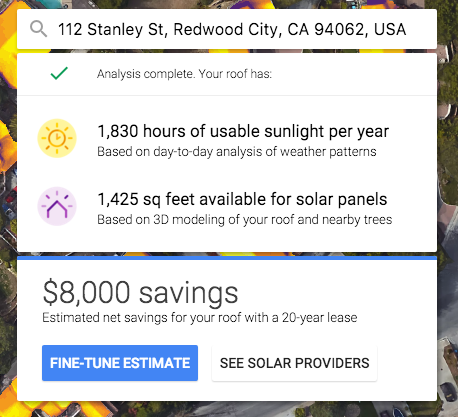
\includegraphics[scale=0.5] {sunroof}
\caption{Project Sunroof analysis and estimated savings for California address with \$100 per month electricity bill}\label{fig:sunroof}
\end{center}
\end{figure}

Though at first Project Sunroof seemed to solve the problem we set out to address, we quickly learned that it falls short in several key areas. When we typed in our own home addresses to calculate the estimated savings, we discovered that Project Sunroof was not available in any of our home states, covering only Fresno, the San Francisco Bay Area, and Boston (Project Sunroof has since expanded coverage to 7 more areas in the United States). Using a sample address, we investigated the calculations Google uses to produce the final recommendation. The algorithm uses a fixed loan interest rate (5.0\%) and assumes a utility electricity price increase of 2.2\% per year \cite{Sunroof}. Furthermore it assumes that electricity consumption will remain the same for 20 years and only permits monthly bill values in \$50 increments. Sunroof sets a seemingly arbitrary upper limit on monthly bill of \$500 (unrelated to available roof area), which hinders utilization for homeowners with more expensive monthly costs. 

As software developers, we saw it as an issue that we could not access the data from the analysis through an API; the results were only available through Google's interface. From our early analysis, Project Sunroof stood out as a rigid, single-interface app. While it does provide an estimate for the home's solar potential in a simple format, it only supports selected areas, uses fixed assumptions, and can only accept a generic monthly electricity bill unadaptable to patterns of electricity use. Despite its good intentions, it leaves gaps in its solution to the problem we set out to address.

Related to Project Sunroof, \cite{Wiginton2010345} explores techniques to determine available rooftop area for photovoltaic deployment. The comprehensive study uses a five-step procedure involving geographic division of the region and shading reduction and, applying the techniques to Ontario, Canada, concludes that 30\% of Ontario's electricity demand could be met with province-wide PV deployment. Studies like this one are important for utility planning, but they do not address individual homeowner interests. The software was used to produce a static result, not published as a tool for homeowners to use for future site evaluations.

In our study of Project Sunroof, we recognized that the overall monthly bill might not provide a complete view of a home's electricity consumption. The DOE released a tool called the Green Button that allows utility customers to download detailed reports of their energy consumption. The initiative is intended to allow the utility customers to take advantage of online applications to help them manage energy use and save on bills. Included in the examples of such applications are products and services for ``sizing and financing rooftop solar panels.'' Although we did not ultimately implement an analysis tool to look at detailed patterns of electricity use as part of the recommendation, our pluggable architecture enables a developer to incorporate a module that analyzes data from a GreenButton report.

In examining available open source data in the solar mapping field, the National Renewable Energy Laboratory (NREL) appeared frequently as a data source in commercial applications. NREL's Solar Prospector is a mapping tool for commercial and utility scale solar projects \cite{Prospector}. Although the prospector does not have rooftop-granularity (instead displaying broad solar potential categories for large regions), it uses other NREL services available through developer APIs. We found services for solar panel pricing, nationwide utility prices, average irradiance values at a specific latitude and longitude, and future performance prediction; these services became core components of our implementation. Although the Solar Prospector does not consider the cost-competitiveness of a solar system by pricing comparison to grid electricity, NREL also has the System Advisor Model (SAM), a performance and financial model designed to ``facilitate decision making for people involved in the renewable energy industry'' \cite{SAM}. SAM is a robust tool that makes performance predictions for solar PV and wind projects. We judged the platform to be overly complex for a prospective rooftop solar owner, intended more for installers than homeowners. 

\subsection{Performance Prediction}
There has been exciting work in the field of solar performance prediction. ~\cite{Iyengar:2014:SCB:2674061.2674071} proposes SolarCast, a cloud-based service that provides customized site-specific predictions of generation for solar deployments. SolarCast uses a "blackbox" approach that requires only a site's geographic location and a minimal amount of historical generation data. While the software can predict future performance of a solar array, it does not give insights into a new installation. However, we identified performance prediction as an important part of our methodology, both to evaluate the success of our approach (by simulating the generation of our recommended array) and, potentially in future development, as part of the recommendation algorithm itself. After contacting the researchers involved with the project, we acquired a key to use the SolarCast alpha API. Although the API is still not yet suitable for our use, our investigation led us to other performance prediction APIs, which we ultimately used to evaluate our approach.

\cite{Bobovych:2015:SHE:2737095.2737110} created a solar panel emulation platform, SunaPlayer, which uses a host of physical electronic devices to build a model of a solar panel. SunaPlayer is intended to aid with solar panel design, not as an evaluation metric for hypothetical installations. Nonetheless, the paper indicates the growing interest in software for solar PV applications. We hope that SunaPlayer and similar initiatives help eliminate doubt surrounding the performance of solar panels, thereby removing a barrier to further growth.

Panel performance prediction is just one half of the equation when determining the long-term cost effectiveness of a solar system. We also must consider the expected behavior of the utility market. \cite{Kjeldskov:2015:EDE:2702123.2702318} built eForecast, which seeks to supplement the data on current and past electricity usage with "eco-forecasting". The prototype forecasts expected usage, electricity price, and expected drops and peaks. It purports to enable people to use electricity at more opportune times. Though we were not granted permission to incorporate eForecast techniques into our algorithm, our framework is adaptable enough to allow future integration. eForecast and other prediction technologies could become important tools to inform our installation recommendation.

\subsection{Real-time Monitoring Systems}
Companies like Bidgely, PlotWatt, and Wattvision monitor home electricity usage with sensors that mount onto electricity meters.  Detailed readings of electricity consumption yield a precise view of the home's usage patterns. Using the electricity data feed, the companies can offer suggestions on improving energy efficiency. While Bidgely can, for example, perform energy disaggregation to distinguish grid electricity from solar, none of these companies evaluate the home's potential to support solar. We recognized that real-time electricity usage data could help construct a more accurate energy profile of the home than the monthly bill. If, for example, the home uses the majority of its electricity after sundown, then recommending an installation to cover 100\% of the home's consumption might be misguided depending on the excess power sellback agreement with the local utility. As a result of this observation, we contacted Wattvision, a Princeton-based startup, and received access to an actual home data stream for testing. Although we were not able to develop an analysis tool more advanced than a simple computation of daily and monthly consumption from a Wattvision data stream, we built the infrastructure to allow a Wattvision plug-in to construct a home energy profile.

Related to real-time electricity consumption monitoring is software for monitoring real-time solar panel performance. Many solar providers including SunPower, Enphase, and First Solar provide APIs and interfaces for their customers to access real-time performance of their arrays. For example, live electricity generation from Princeton University's solar array is available through SunPower's API and visualized in the Office of Sustainability's Tiger Energy application (\url{http://www.wattvision.com/princeton/solar}). After surveying solar systems, we chose the Enphase Enlighten system as the one for further analysis because of its extensive API. The Enlighten API has endpoints to fetch current production, total monthly production, and power per area \cite{Enlighten}. Although the API is principally intended for Enlighten customers to access their own data, Enphase provides a mechanism to allow third-party developers to request access to data feeds. We reached out to a member of the Enphase developer team, who identified a group of candidate systems that could produce an accurate estimate for the power output of a hypothetical array. We are currently awaiting final approval to send out authorization requests, which will allow us to make API requests on behalf of homeowners to access their system data.

Considering the related work we investigated, we identified Project Sunroof's simple model as an ideal medium for conveying the solar potential calculation to the homeowner. Similar to Project Sunroof, we chose cost savings and installation size as the two key values to report to the user. From related fields including solar performance prediction and real-time monitoring software, we understood the value of exposing an API, which allows others developers to leverage our analysis tools. When we began work on SolarSource we recognized three areas as missing from previous efforts in achieving our goal: universal coverage for homeowners, framework flexibility, and incorporation of actual generation data. This led to our approach.

\bigskip
\bigskip

\section{Approach}
Our goal to create a universally applicable and accurate framework to estimate home solar potential suggests the following approach, composed of five key ideas.

\subsection{Decoupled Back End}
To enable widespread and flexible use of the framework, we build the back end of the framework as a standalone API conforming to REST protocol. The benefit of such an approach is flexibility. With a publicly accessible API and a comprehensive JSON return output, anyone with knowledge of HTTP can make requests to the API to use our analysis tool, either a developer writing a front-end application or even a homeowner with specialized knowledge of her roof plan. The information we can provide is not limited to users of our front end application, as is the case for similar solar calculators.

\subsection{Adaptable Architecture and Open Source}
All of the software-for-solar apps we discovered in our research hide their implementations; we set out to create a useful tool for both homeowners and the developer community. To do that we open-source the code on Github in a public repository and design the software to incorporate plug-in modules. The benefit of this approach is that it promotes transparency and enables future development. With our code on Github, we provide transparent access to our methodology and data sources. More importantly, any developer can build on the work we started, augmenting the framework with custom modules or displaying it in a specialized interface.

\subsection{Universal Coverage: Do-it-Yourself Home Profile}
An accurate model of the home is the foundation for any type of energy upgrade including a solar installation. Our goal is to provide {\em every homeowner} with the tools to determine the home's solar potential - to achieve that goal we need to make the framework universally usable. After surveying previous work, we realized that we could construct an accurate profile of the home with user-supplied data on roof properties and electricity consumption. This technique permits the framework to be used anywhere with internet access, unlike Project Sunroof, whose utilization depends on Google's choice of coverage. Providing the user with the tools to profile the home severs our dependence on potentially out-of-date map APIs and electricity data. For example if a homeowner has recently built an extension to the home, an aerial image might not depict the current roof, leading to an inaccurate estimate of solar generating potential.

\subsection{Leverage Third-Party APIs}
In order to determine the generating capacity of a rooftop solar PV system, as well as the price of that system, we need data on panel prices and sunlight availability at a specific location. Previous efforts have relied on proprietary data. Yet to achieve our goal of both an accurate {\em and} adaptable framework, we require data that is both reliable and publicly accessible. From our study of NREL's Solar Prospector application, we learned that much of the data we needed is openly available through NREL's developer API. We therefore use NREL's datasets as the core informational foundation of our recommendation analysis. This decision has two key benefits. Firstly, as a governmental facility that has contributed to renewable energy developments since 1974, NREL is a reputable and reliable source. Secondly, the data is openly available; this allows other developers to augment our framework (by forking the project on Github, for example) without worrying about proprietary access issues.

\subsection{Crowdsource Power Generation Data}
We use actual generation data when estimating the production of the recommended array. The accuracy of the recommendation relies heavily on the power output of the array. Some services use generic industry-reported values (1 kilowatt per square meter, for example) for a panel's output. However, production values vary depending on environment. Rather than using a fixed value, the output of the recommended array is computed using past performance of existing arrays in similar environments. Using crowdsourced data from real installations close to the target address allows us to get a more realistic view of how the panels would perform in practice.

\bigskip
\bigskip

\section{Implementation}
\subsection{Breakdown of Work}
The work on SolarSource is divided into three areas among our team (composed of Emily Speyer, Gregory Magana, and myself): roof profiling, core Android application, and back end API. We chose a mobile app for the front-end interface to facilitate ease of use and to take advantage of phone features like compass, camera, and GPS.

Emily implemented the roof profiling system as a standalone Android application, outlined in \cite{Speyer}, that integrates with the core app. Using the application, the user maps out the roof's area by walking around the perimeter of the home. The program factors in shade and other obstructions to the roof to compute the usable roof area along with tilt angle and orientation. The roof profile provides the physical constraints for an installation and necessary parameters to determine how much electricity a hypothetical rooftop-mounted PV system could produce.

Gregory built the main Android application described in \cite{Magana}. It accepts user input on monthly electricity bill, delegates control to the roof profiling stage, and communicates with the RESTful API backend to compute and display the final recommendation. The application enables our usage of a Wattvision data stream by allowing the user to provide a Wattvision system identification number with which the back end can make requests to the Wattvision API. The home energy profile, created with data sent through an Android application, determines the ideal array size and cost-effectiveness of the proposed  system. 

I implemented the back end API, which uses data from the front end to produce a recommended installation size and performs the cost analysis. First I will explain the high level design decisions behind the API implementation. Then I will give an overview of the process flow, discussing each step individually. 

\subsection{System Architecture}

\begin{figure}[h]
\begin{center}
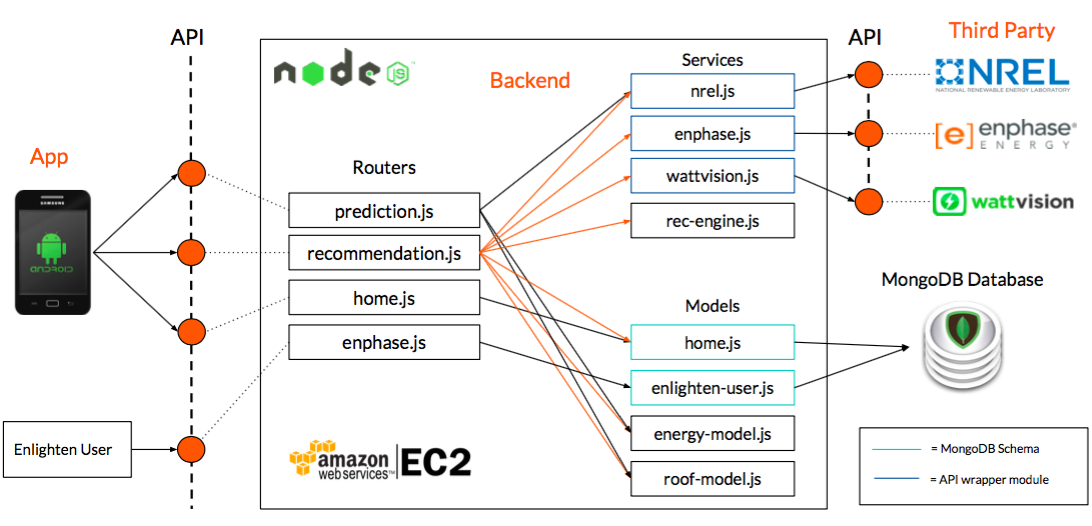
\includegraphics[width=\textwidth] {architecture}
\caption{High level system architecture}
\label{fig:architecture}
\end{center}
\end{figure}

Figure \ref{fig:architecture} shows a high-level illustration of our architecture. The basic structure is as follows: we expose an API with endpoints to create and operate on a home model ({\em /api/homes}) and to retrieve the solar array recommendation and cost estimate ({\em /api/recs}). The codebase consists of three main file categories: routers, services, and models. Routers handle the HTTP request logistics, perform input validation, retrieve objects stored in the database, and call service methods. We give each API group its own router to promote modularity. The models consist of both database schemas (descriptions of database entries) and home models created with input from the user. Services include wrapper modules to call third party API methods and the recommendation engine, which computes the necessary array size and performs an economic analysis to estimate savings. We store all home objects in a database. We used MongoDB for the database layer and deployed the application to an Amazon Web Services EC2 instance. We use a configuration file (not shown) to store API access keys, endpoint URLs, and constants.

Our architecture presents opportunities for developers to write custom analytics tools in such areas as Wattvision stream parsing, electricity price forecasts, and future consumption predictions based on current patterns, an alternative to assuming constant consumption for 20 years.

\subsection{Platform and Web Framework}
Our goal in this step was to find an API development platform that promoted adaptability, facilitated HTTP routing, and was enjoyable to program with. Popular approaches include Python (with the Django web framework) and Node.js (a Javascript-based runtime environment). To achieve the flexibility goal from our approach we require a platform that supports easy integration of custom modules. With that consideration, Node.js is the clear choice for its modular design and robust package manager, npm. Every file in Node is a module with associated methods and instance variables. Node's design aligns with our need to allow developers to plug in their own code without modifying large chunks of the original codebase.

With Node, installing an external package is as simple as one npm command; importing the package (or an internal module file) entails initializing a single variable, which scopes the entire package to that variable, a major benefit in light of Javascript's exclusively global namespace. As our first step, we downloaded the Node package using the OS X package manager Homebrew.

Developing the API calls for a web framework to supplement Node.js. Our goal in this step is to maximize code readability to facilitate future augmentation. In choosing a web framework, we consider not only syntax but also popularity; the time it takes to read documentation on an unfamiliar framework may hinder a developer's understanding of our code. We experimented with several popular and well-reviewed frameworks (writing basic route handlers with each one) including Loopback, Sails, and Express. Express is the most popular Node framework on Github and used in production by Netflix. Its documentation contains many useful code examples. Loopback is a heavy-duty framework, providing features like automatic API documentation and support for Android applications. However, it is bloated with highly specialized functionality and convoluted syntax. More importantly, the documentation is difficult to understand, a key drawback for our readability guideline. Sails is inspired by Express and extends it for front end functionality. It is a full model-view-controller framework, intended for use by MVC applications. Given that the back end is solely an API, we have decided to use the more minimalist Express, which we also judged as the most straightforward in our basic experimentation. We used the npm package express-generator to create an Express template for the application. The template separates route handling functions in a separate directory, a structure we adhered to throughout development.

\subsection{Callbacks vs Promises} 
Javascript is an asynchronous language. I/O calls, database lookups and API requests do not block execution; instead execution jumps to the next line. To deal with this language feature, most programs make extensive use of callback functions, whereby you pass a function as an argument to an asynchronous method. The function is called with the response of the asynchronous request. As we read tutorial code, we decided that function callbacks make code difficult to understand. When asynchronous calls are deeply nested, they can produce the dreaded and unreadable ``pyramid of doom'' as shown in Figure \ref{fig:callback-hell}.

\begin{figure}[h]
\begin{center}
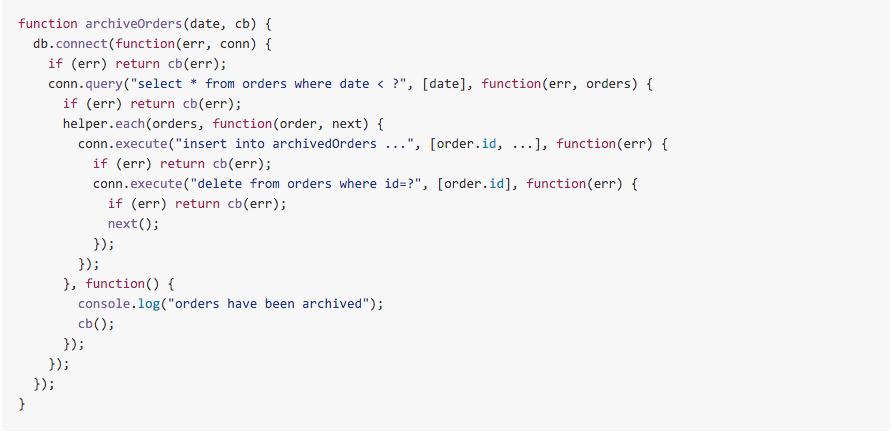
\includegraphics[scale=0.5] {callback-hell}
\caption{Pyramid of doom whereby the function grows outward as a result of many nested callbacks}
\label{fig:callback-hell}
\source{https://github.com/Sage/streamlinejs}
\end{center}
\end{figure}

Our code is open-source and intended to be augmented by other developers. It therefore needs to be easily understood; readability should be the rule. Our goal in writing asynchronous Javascript is to maximize readability. With that goal in mind, we determined that we couldn't use callbacks. 

There are numerous Node libraries to circumvent callbacks. We have surveyed the options by reading code samples to gauge comprehension and ease of use. The two primary high-level approaches to combat the callback model are callback replacement and promises. Callback replacement involves replacing the callback function with a special symbol and writing the code as if the function is synchronous. The replacement library handles the asynchronicity behind the scenes. 

Promises are a concurrency primitive that essentially `promise'' that a value will be there when you need it or the method call will fail entirely. The returned value of an asynchronous function is a promise, which is ``thenable'', meaning that a method can be called on it with the resolved promise value passed as an argument. In English, one might describe thenable execution as ``return this value, then operate on it.'' To make this design clearer, Figure \ref{fig:promises} is a code excerpt illustrating how callbacks might be transformed with promises.

\begin{figure}[h]
\begin{center}
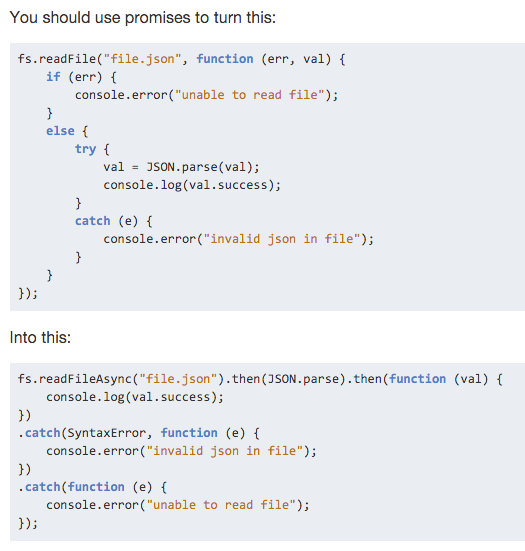
\includegraphics[scale=0.4] {promises}
\caption{Illustration of how promises help with writing flat code}
 \label{fig:promises}
\source{bluebirdjs.com}
\end{center}
\end{figure}

After evaluating the two approaches on such metrics as popularity, readability, and functionality, we have decided to use promises, primarily because they will become part of the Javascript language in its next official release, ECMAScript 6. With promises as a core language feature, we judged it to be more likely that a Javascript developer would understand our code without needing to consult dense reference documentation.

Promises are a design philosophy - the actual functionality is implemented in special-purpose promise libraries built by third party developers. Among the most commonly used third-party libraries are Q, D, and Bluebird. D lacks useful features beyond the core promise implementation. Both Bluebird and Q have extensive reference documentation. Due to Q's error handling, exceptions can go unobserved at the end of promise chains. Bluebird on the other hand reports all errors without special syntax and displays helpful stack traces for error detection. In addition, Bluebird has zero overhead abstraction, meaning that we can use its features without sacrificing performance. Bluebird emerged as the best option, also providing helpful methods for operating on promise values (for example, with a {\em map()} function) in line with promises chains. In our codebase, we make frequent use of Bluebird promise chains in which each step in the chain returns a promise. Every asynchronous API wrapper method returns a promise. Any time we call an asynchronous method, including database queries and wrapper method invocations, we wrap the return value in a promise handler to keep our code flat.

\subsection{Documentation}
Clear documentation is necessary in order to enable general-purpose use of our API (and to facilitate our front end development process). Our goal is to inform API clients of the exact parameter requirements of each API method and the expected return values, establishing the contract between caller and callee. Several methods are possible for generating documentation, including Github wiki and the Node.js package, apiDoc. With Github, the documentation is included with the project code, a benefit for convenience. However, Github's editing platform for project wikis makes it difficult to include JSON samples, which are essential for describing HTTP request body syntax. apiDoc, on the other hand, allows you to create API documentation with Javadoc comments directly in the code file. You can include JSON samples easily, and generating the documentation page is one command line instruction to compile the Javadoc comments. The created page is interactive, legible, and visually appealing. Considering these tradeoffs, we have chosen to use apiDoc and host the generated documentation page using the Github Pages hosting platform. For each API method, a Javadoc comment specifies endpoint descriptions, required parameters, return status codes, and example JSON request and response bodies. Figure \ref{fig:apidoc} shows the top of the documentation page, which can be found in its entirety at \url{http://g2-iw.github.io/backend-iw/}. With the API fully documented, the back end services can operate independently of the Android app. The SolarSource app is just one client of the API; anyone can use the back end services to determine the viability of a rooftop solar installation.

\begin{figure}[h]
\begin{center}
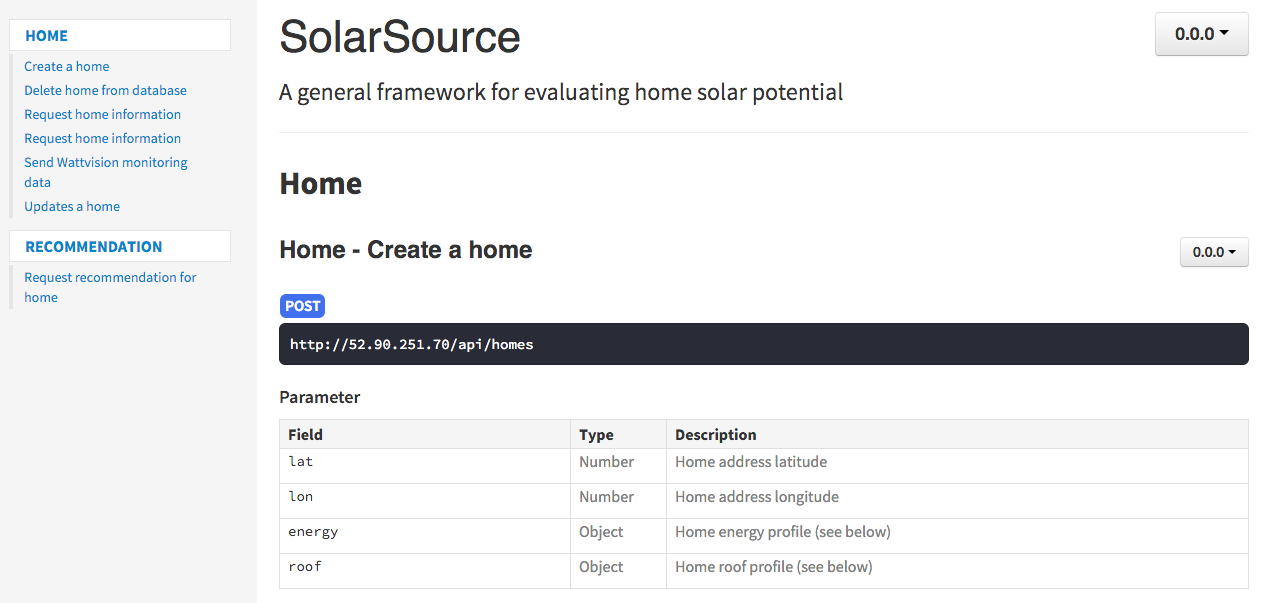
\includegraphics[width = \textwidth]{apidoc}
\caption{SolarSource API documentation page created with apiDoc}
\label{fig:apidoc}
\end{center}
\end{figure}

\subsection{Database Layer}
For the purpose of returning a recommendation, it is not strictly necessary to store home objects. The back end could simply perform the evaluation from start regardless of whether the home has been profiled before. However, we want to enable using performance data from profiled homes (i.e. a homeowner installed panels based on the SolarSource recommendation) as part of the crowdsourced platform to inform future recommendations. In addition, we recognize that the third party API requests are costly - if we have already performed an analysis for a home it is unnecessarily time consuming to go through the process again for the same home. We therefore store home objects in an application-attached database. In choosing a database, our goal is to make database operations as seamless as possible; given that database storage is a performance improvement and not a core component of the analysis, it should not bloat the code. Possible approaches include MongoDB, Hadoop, and Redis. We use MongoDB because it uses JSON-like documents to store database entries rather than relational tables. The JSON documents are compatible with regular Javascript code without much processing. With MongoDB we are also able to use the Mongoose library, which supports promises. We have created a MongoDB database and connected it to the application. Schema files describe the structure of home database documents. Database query and document creation code live in the route handlers.

\subsection{Deployment}
Our goal in this stage is to deploy the API to a stable, reliable server that supports external volume storage. We opt to deploy to a cloud server because of simplicity and low cost. Several approaches exist for cloud application deployment, including Amazon Web Services (AWS), Digital Ocean, Heroku, and Google App Engine. We have chosen AWS because it allows free deployment under a certain usage limit and provides an instance machine image preloaded with the Node.js and MongoDB environments. A custom security group allows all members of the SolarSource team to SSH into the cloud instance. We use a key pair for encrypted sign-in. Deploying the application entails first launching an Elastic Compute Cloud (EC2) instance with the desired machine image. After developing and testing the API locally, we pull the code from Github on the cloud instance, configure the production database, and start the server with the Node.js Forever library, which keeps the server running after you break the pipe with the remote instance.

\bigskip

\subsection{High Level Process Flow Overview}

\begin{figure}[h]
\begin{center}
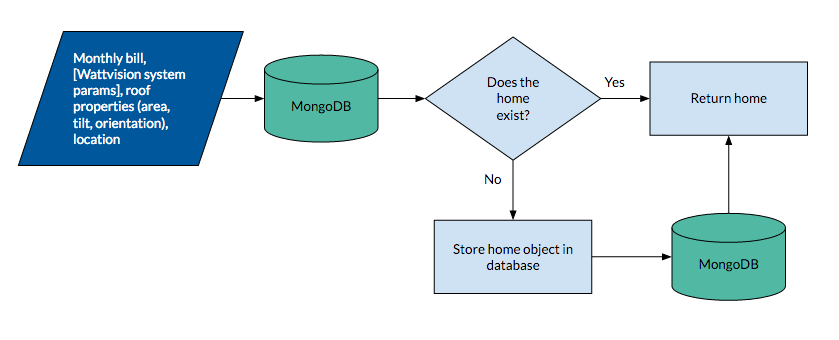
\includegraphics[width= \textwidth]{POST}
\caption{Home creation POST method}
\label{fig:post}
\end{center}
\end{figure}

\begin{figure}[h]
\begin{center}
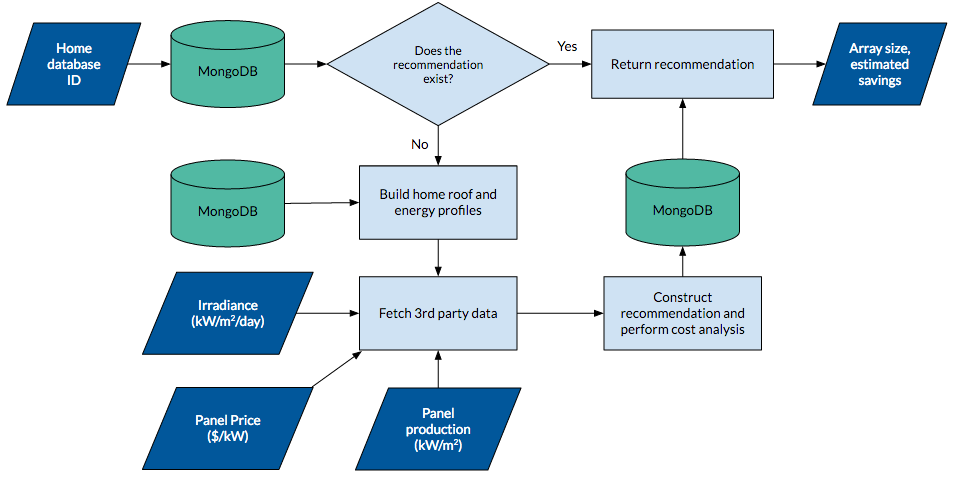
\includegraphics[width=\textwidth] {GET}
\caption{GET route to retrieve recommendation and cost savings estimate}
\label{fig:get}
\end{center}
\end{figure}

We first outline the flow of control to generate an array recommendation and cost savings estimate for a home. Figures \ref{fig:post} and \ref{fig:get} illustrate the processes. The process begins with an HTTP POST request to the {\em /api/homes} endpoint. The input to our system is home energy consumption (in dollars per month), optionally the Wattvision system identification number, and the roof properties: usable area, tilt, orientation (compass direction), and azimuth angle. All inputs are passed in the body of the request. In the handler method for the POST request route, we store the home in the database if it does not yet exist and return the created home JSON object. 

To access the recommendation for that home, the client then makes a GET request to the recommendation endpoint {\em /api/recs}, passing the home's database ID as a query parameter. If the home's recommendation has already been computed, the route handler returns the existing recommendation. Otherwise the method constructs the home profile from the user data and retrieves the necessary information from third party APIs. It then passes all the necessary information to the recommendation engine module. The recommendation engine computes the recommended solar array size and performs the cost comparison analysis. The router formats the recommendation and returns a JSON object to the client with the recommended array size and estimated savings. Figure \ref{fig:output} shows a sample JSON output. The following subsections describe each of these steps in detail. We separate the home creation endpoint from the recommendation retrieval so that a user can easily access the recommendation of a previously used home without the unnecessary steps of the POST creation method.

\subsection{Home Creation}
In the first stage, the client makes a POST request to the API. Our goal is to convert the user-passed JSON object into a home database entry and store it in the database. The inputs are the monthly electricity bill, optionally Wattvision system identification numbers, and roof properties from the user-generated mapping. For this simple handler, our approach is largely determined by our decisions to use MongoDB and promises. However, there is freedom in our choices of file layout and parameter passing. One approach is to mount the handler function directly onto the main route of the application. This would be done in the {\em app.js} file, which starts the server and configures the application properties. Another common Express approach is to create a separate router file (a module), and append route handler functions to the router module. In the {\em app.js} file, you mount the entire router onto the application rather than the individual methods.

We employ the latter approach for two key reasons. Firstly, it is less error prone; rather than writing the same style code to mount multiple methods in the same API group, we only need to mount the router once. Using the router modules has the added benefit of clarifying the API structure; each router has a one-to-one mapping with an endpoint group. The router modules effectively package related route handlers. Secondly, it encourages decoupling of components. In this and other aspects of the codebase we strive to decouple components to the largest extent possible. Decoupling enables easier module swap-in and modification without breaking other parts of the code; service components can be swapped out without changing the routers at all, so long as they use the same parameters. A potential workaround to this parameter problem is foregoing input validation in the router and sending a full Javascript object to the service or database layer as an argument (in that case, the home database schema would be a generic and mutable empty object). Service layer code would have the responsibility of retrieving the necessary fields from the home object. We opt not to do this because it risks safety - the user can pass anything in a request body. We prefer a strict structure for the home database schema to enable MongoDB to perform internal input validation.

We create a separate router file for the home. Within the router file we have a separate route handler for each CRUD (creation, retrieval, update, and deletion) operation. Although the Android application only makes a POST request, the other handlers facilitate testing and are useful for general API access. Figure \ref{fig:postrouter} shows how we implemented the route handler for the POST method.

\begin{figure}[h]
\begin{center}
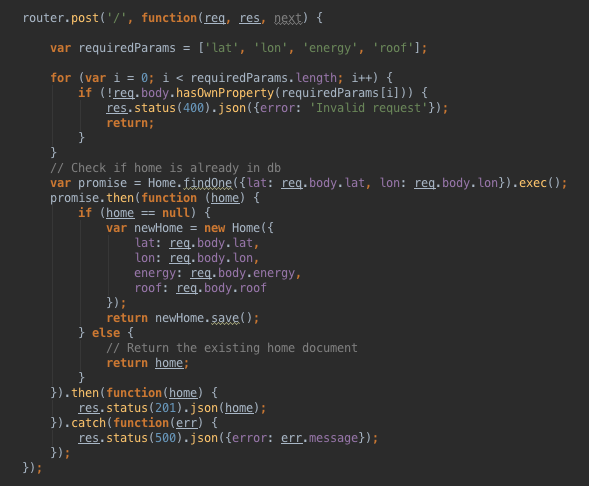
\includegraphics[scale=0.5] {postrouter}
\caption{Route handler for home POST method}
\label{fig:postrouter}
\end{center}
\end{figure}

We first verify that the caller has supplied the required parameters. Using promise syntax, we query for the home in the database by latitude and longitude in case it has already been created. If so we retrieve the database entry and return it immediately. Otherwise we create a new home document with properties equal to the request body attributes. We then save the home in the database and return the database entry to the caller to indicate to indicate the process was successful.

In this and all other HTTP methods, we strictly adhere to the model of: perform input validation, query the database for an object or create a new object, and return a JSON object to the user, either an error description or the result of the successful database operation.

\subsection{Recommendation and Cost Analysis}
In the second stage, the client makes a GET request to the recommendation endpoint, using as a query parameter the database ID returned in the POST response body. If a recommendation has not been created for this home before, then it begins the analysis. The overall goal of this stage is to return an accurate recommendation for an array size to cover a percentage of consumption and estimated cost savings due to the recommended array. The inputs to this stage are home energy and roof profiles, utility electricity rates, solar irradiance, panel price, and array generating capacity, the latter four of which come from third party API requests. We will discuss each step individually. 

For the overall structure of the recommendation route handler, a common approach for a handler that makes many asynchronous requests is to use nested callbacks. However, as previously discussed, deeply nested callbacks contradict the design goals from our approach. This is an ideal use case for a Bluebird promise chain. At each step in the process, we retrieve data that ultimately gets passed to the constructor of the recommendation engine module. The promise chain ensures that the data is available when the engine object is instantiated. The promise chain also allows us to write flat, readable code, with each component of the promise chain performing a well-defined task. Rather than using global variables to store the result of each external method call, we use one context variable, a Javascript object, bound to the promise chain. At each stage we append a new attribute to this dictionary object.

The recommendation route handler illustrates how we separate HTTP routing from the analysis tools entirely, adhering to our decoupling principle. The logic is abstracted away in the service and model levels, while the router performs the necessary linkage operations.

\bigskip

\subsubsection{Construct Home Models:}
The goal of this step is to construct models for home energy consumption and roof availability using data passed by the client in the first phase. The models provide access to properties required for third party API calls and the cost analysis. Such properties include total usable available roof area and average monthly electricity consumption. In the simple case, the data passed by the  the client in the POST request is sufficient for the profiles. One possible approach, therefore, is to simply retrieve the necessary attributes from the home database entry. An alternative is to create separate modules for the roof and energy profiles and only provide access to the necessary data through an interface.

We use the latter approach in anticipation of another developer adding methods to operate on the user-inputted data for more advanced analyses. For instance, if the user grants access to his Wattvision data stream, we could construct an energy model to analyze patterns of consumption. Rather than using data straight from the home database object, we retrieve home information only through the models' interfaces. That way, we can do more advanced computation behind the scenes without changing the calling code and still return the necessary information to the caller through {\em getEnergyProfile()} and {\em getRoofProfile()} functions.

In the recommendation route handler, we call the constructors for the energy and roof models, passing in the matching objects from the home database objects and, in the case of the energy model, an optional Wattvision data stream. We fetch the Wattvision data in the recommendation handler (rather than the energy model itself) because we wanted to have all external API requests in the same place. This helps prevent potential asynchronicity issues. The models' constructors call the analysis methods so that the caller can simply call the constructor.

The roof model comprises such properties as square footage, roof tilt, and geographical coordinates. Information from the roof model determines the physical constraints for an installation and subsequently the maximum power generation. For the energy model, we perform an analysis using measurements taken by the Wattvision sensor if the home has one. Otherwise we compute the monthly consumption value by dividing the monthly cost by the standard dollar per kilowatt-hour cost retrieved from NREL's Utility Rates service. The home's electricity use determines the required array size to cover a portion of the home's consumption. In our current implementation we recommend an array to cover close to 100\% of the home's consumption. However, we provide the flexibility to change that percentage in a configuration file or plug in a custom tool to determine the most cost effective installation size given patterns of usage or electricity price forecasts. At this step we have the maximum size of the array and the required array production to match a specified consumption amount. 

After the constructor calls return, the recommendation route handler retrieves the home and energy profiles through the model interface methods {\em getRoofProfile()} and {\em getEnergyProfile()} and appends the profile objects to the context variable.

\bigskip

\subsubsection{Retrieve NREL Data:}
In the next step, our goal is to retrieve the necessary NREL data to generate an installation recommendation and perform the cost analysis. We want to do this in a way that does not disrupt code readability. The required inputs are the home's coordinates, roof tilt, and roof azimuth angle. The desired outputs are price of panels (\$/kW), utility rates (\$/kWh), average solar irradiance at the coordinates (kWh/$m^2$/day), and panel production (kW/$m^2$). We discuss acquiring panel production data in the next section.

In this step we face the issue of calling external NREL API endpoints. One approach is to call each method directly when needed in the route handler. However, that would require complicated callback code and entangle the router logic with boilerplate HTTP request syntax. We took an alternative approach; we use entirely separate modules to call external API methods. In these modules, we have an individual method for each endpoint we need to hit. We use the Superagent library to construct the requests. Superagent provides simple syntax for specifying query parameters, request headers, and response format.

These methods accept home properties from the energy and roof models as arguments, which are passed as query string parameters in the HTTP requests. Each method returns a Javascript promise object to facilitate integration into the promise chain. With this approach, our route handler calls a method from the wrapper module in one-line and receives the formatted response with the necessary data. We call the Solar Resource Data service for average solar irradiance, OpenPV for panel price, and Utility Rates for electricity prices. The router appends the returned data onto the context variable. Figures \ref{fig:nrel-wrapper} and \ref{fig:nrel-call} show an example of one wrapper method for the NREL Solar Resource API and how it gets called in the route handler:

\begin{figure}[h]
\begin{center}
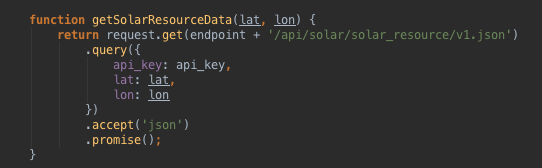
\includegraphics[scale=0.6] {nrel-wrapper}
\caption{Wrapper function to make HTTP request to NREL API}
\label{fig:nrel-wrapper}
\end{center}
\end{figure}

\begin{figure}[h]
\begin{center}
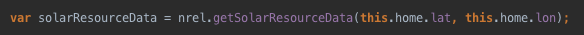
\includegraphics[scale=0.6] {nrel-call}
\caption{Wrapper function call in the recommendation router}
\label{fig:nrel-call}
\end{center}
\end{figure}


\subsubsection {Acquire Generation Data:}
Our approach calls for the use of actual data in place of fixed values to compute the peak power output of a hypothetical array. Perhaps our most difficult challenge, and the goal of this step, is to collect accurate solar panel generation data. The two types of generation data are static and dynamic. Static data is normally downloadable, a spreadsheet of generation values over a certain time period. Dynamic data is retrievable in real time via API request. It provides the current power production of the solar array along with past data.

We have elected to use dynamic data to avoid bloating the codebase with large data files that would need to be manually updated periodically. With dynamic data, we can make on-demand HTTP requests and use the most up-to-date data in the analysis. The application does not store the data, instead retrieving it ``on the fly.''

Our options for dynamic generation data are severely restricted by what we can gain permission to use. Often generation data is proprietary and protected. Given our extensive use of NREL's services, we reached out to try to gain access to generation data. After speaking with Principal Scientist Sarah Kurtz, we were given an API key for the Photovoltaic Data Acquisition (PVDAQ) service, which provides access to PV performance data collected by NREL for systems throughout the country. Endpoints of the service return generation data for each site including monthly generation, array area, and power output readings at regular time intervals similar to Wattvision meter readings.

By means of a wrapper method call in the route handler, we query the PVDAQ database for systems within an adjustable radius of the target home. We compute an average power per area across the collection of PVDAQ systems for the value used in the analysis and append the value to the context variable. 

Most of the PVDAQ systems are large commercial installations. Even though the total size of the installation should not effect the power per area value, we thought it would bolster the accuracy of our recommendation if we also used generation data from residential solar arrays as part of a sort of a crowdsourced platform. From our survey of related work, we selected Enphase as our target system for generation data. The Enlighten API has well-documented endpoints to access site metadata, current production in 15-second intervals, and total monthly production.

We contacted Benjamin Smith on the Enphase developer team and requested access to Enlighten system data. Mr. Smith identified candidate systems he thought would be representative of actual generation in Long Island, New York, where we would ultimately conduct our evaluation experiment. We are waiting for final approval to send out emails to the owners of those systems, in which we describe the purpose of our project and request access to their API keys so that we could make requests on their behalf. Currently we are not using the Enlighten system data, but we have created wrapper methods to integrate those data feeds into the analysis once we gain authorization from the owners. 

\bigskip

\subsubsection{Calculate Recommended Array Size and Capacity:}
The goal of this step is to use the precomputed data from the home profiles and third party API requests to calculate an array size to cover a configurable percentage of the home's consumption. The desired outputs are the hypothetical array properties: area (in square meters) and power (in kilowatts). The desired outputs determine the calculations to be performed. Approaches differ in where to perform the calculations, within the recommendation route handler or in a separate module. We chose to create a separate module to compute the recommended array size and cost analysis, which we call the {\em recommendation engine}. Our decision is based on adherence to modular design. We want to enable easy swapping-in and swapping-out of components, including the array size and cost estimate calculations. Within the recommendation engine, one option is to encompass all functionality within the constructor. However, we found that each component of the analysis could potentially call for its own tool. Striving to maximize modularity, we break up the logic into small, well-defined parts, thereby extending our principle of decoupling to within files as well as the file structure. We divide the array size and cost estimate computations into four functions:

\begin{itemize}[leftmargin=1in]
\item calculateArraySize()
\item calculateArrayCapacity()
\item calculateArrayCost()
\item performCostComparison()
\end{itemize}

The route handler instantiates a recommendation engine object, passing the context variable as an argument. From the home energy model, we know the required array production to match the home's consumption. To convert from that value to array size, the constructor calls the method, {\em computeArraySize()}, which multiplies total consumption $c$ by the desired coverage percentage $d$, and divides the result by the average solar irradiance value at the site, $i$. Irradiance is a measure of how much sunlight the site receives. We call the analysis methods from within the constructor so that the caller only needs to retrieve the result of the analysis after the constructor returns. If the array size exceeds the maximum usable roof area, we set a flag set and set array size to the maximum allowable size. We save the array size and coverage fraction (what percentage of home consumption the array covers).

To calculate array capacity, the constructor calls the {\em calculateArrayCapacity()} function, passing the array size. In this method we leverage the crowdsourced generation data, multiplying the array size $s$ by the average power per area value $p$ computed in the previous step to yield a peak power output for the array.  At this point we know the array size and maximum capacity to generate the required amount of electricity. Here are the formulas we use:

\begin{align}
s \text{ ($m^2$) } &= \frac{c \text{ (kWh/month) } * d \text{ (\%) }} { i \text{ (kWh/$m^2$/month) }} \\
\text {array capacity (kW)} &= s \text{ ($m^2$) } * p \text{ (kW/$m^2$) }
\end{align}

\subsubsection{Perform Cost Comparison:}
The goal of this step is to compute the cost of the array and compare the economics of solar to projected grid electricity costs. The required inputs are the monthly electricity bill and hypothetical array capacity and size. The desired outputs are the array cost and projected savings (or losses) from the solar installation.

From a high-level perspective, one approach is to create a separate module for the cost analysis. Although that approach fits our modularity mandate, we encapsulate the cost comparison within the recommendation engine because the cost analysis requires the hypothetical array properties. From the constructor we call {\em calculateArrayCost()}, passing the array capacity computed in the previous step. We multiply the array size by the regional average panel price (\$/kW) from the OpenPV service. We assume the panel is purchased via a 20-year loan, the most common solar financing option. Thus for the total cost of the system, we multiply the upfront cost by the compounded loan interest over a 20-year period. For the loan interest rate, we assume 8\%, although the value can be modified in the configuration file or determined via a custom projection tool. We assume that excess electricity generated by the array can be sold to the grid at the same price it is purchased for; the grid serves as a ``battery.'' As long as the array's monthly production equals home consumption, the electricity purchased from and sold to the grid cancel, so the only cost is the monthly loan payment. If the hypothetical array does not cover all of the home's consumption, we add the balance for grid electricity cost to the array cost.

In the next step, the constructor calls {\em performCostComparison()}, passing as an argument the array cost. To determine the cost savings, we first compute the projected electricity costs assuming the home uses only grid electricity. For the basis of the projection we use the home's current monthly electricity cost $m$, either the user-specified bill or the product of monthly consumption from a Wattvision analysis and cost per kWh retrieved from the NREL Utility Rates endpoint. 

The goal of this sub-step is to accurately compute the 20-year electricity cost. Without a reliable source to project consumption trends, we decided to assume that consumption remains constant. By retrieving the consumption change via separate method call, we provide the flexibility to swap in a custom module to project consumption changes. For electricity price increase rate, $r$, we chose to use Project Sunroof's assumed value of 2.2\% per year. Again in this case, we retrieve the price increase rate via method call, providing the option to write a custom projection module. The following formula shows the computation to arrive at 20-year electricity price:

\[ \mbox{20-year cost (\$)} = m \mbox{ (\$/month) } * \mbox{12 months/year} * \mbox{20 years}  * (1+ r)^{20} \]

We compute savings by taking the difference of the 20-year grid electricity costs and the price of the loan-financed solar array. Here we accept that modern solar arrays use micro-inverters and should require no maintenance (and therefore no additional cost) during their first 20 years \cite{Sunroof}. The handler retrieves the array size and cost analysis values through the recommendation engine object's  {\em getRecommendation()} method and appends the output to the context variable. In a for each loop, the handler then appends each recommendation data field to the original home database object so that the recommendation can be easily retrieved in a future request. Finally the handler saves the updated home object and returns the recommendation object to the client, whose format is shown in Figure \ref{fig:output}.

\begin{figure}[h]
\begin{center}
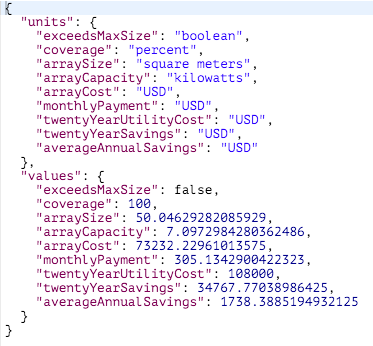
\includegraphics[scale=0.6] {json-out}
\caption{JSON object returned by recommendation GET request handler}
\label{fig:output}
\end{center}
\end{figure}


\section{Evaluation}
We have executed a set of experiments to test the accuracy of our implementation's recommended generation and cost savings. To evaluate how well we achieved our goal of generality, we perform a qualitative analysis on several key principles against Project Sunroof.

For our first experiment we profiled a home in Princeton with solar panels already installed. After generating an installation recommendation for the home, we can evaluate our implementation's accuracy by comparing our projected savings to the actual savings from the solar array, extrapolated to align with the 20-year loan. The inputs to the experiment are the home roof properties, home address, and monthly electricity costs.

To conduct the experiment we manually mapped out the roof using a tape measure, which yielded an area of 48.02 meters and a tilt angle of 30 degrees. We obtained the past two years of PSEG monthly electricity bills from the homeowner; the solar installation came online in March 2015. Using the Postman HTTP client, we first store the home in the database via the homes POST method, passing the home data in the request body. From the past electricity data, we ascertain that the array covers 63\% of consumption. Therefore, for the monthly electricity cost we use 63\% of the pre-installation monthly bill. We make a GET request to the recommendation endpoint with the home's ID as a query parameter to perform the analysis and retrieve the recommendation. The response JSON object is shown in figure \ref{fig:blejwas}.

\begin{figure}[h]
\begin{center}
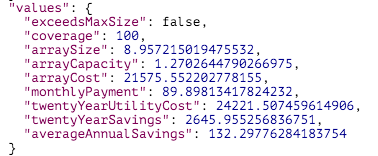
\includegraphics[scale=0.7]{blejwas}
\caption{Installation recommendation and cost savings estimate for Princeton home with solar panels installed}
\label{fig:blejwas}
\end{center}
\end{figure}

To compute actual savings due to the array, we first take the difference between average monthly cost before and after the panels were installed. We extrapolate twenty-year gross savings from the reported savings by assuming consumption remains constant and the electricity price increases by 2.2\% per year. From that value we subtract the installation cost. 

Extrapolating from reported savings yields total 20-year savings of \$4221. The SolarSource recommendation estimates savings of \$2646, an error of -37\%. We attribute the high error to an overestimation of solar irradiance at the site by NREL Solar Resource service. The recommended array size is the home's monthly consumption divided by solar irradiance. Figure \ref{fig:blejwas} reports a recommended array size of 8.96 $m^2$. However from visual inspection of the roof, the panels cover an area close to 20 $m^2$. Perhaps other methods for computing site irradiance would produce better results.

One home is of course a small sample size. We were limited by access to electricity billing data for homes with panels already installed. In future experimentation, we would use this evaluation model on a wider scale. 

\subsection{Quantitative Comparison to Project Sunroof}

Our second experiment tests how well our implementation performs against Project Sunroof. We chose Project Sunroof because it is a direct comparison application whose features motivated our approach. By running both analysis tools on the same set of homes, then comparing the results to projected panel performance and cost savings, we can evaluate the accuracy of our implementation compared to Google's on the metrics of recommended array production and cost savings. Similar to the first experiment, the inputs to this experiment are home address, home roof properties (for SolarSource only), and monthly electricity cost.

To compute the projected performance and savings, we use NREL's PVWatts service. PVWatts estimates the performance of hypothetical residential and small commercial PV installations given latitude and longitude, tilt angle, and system capacity. The response object contains three arrays: monthly irradiance values (strength of solar energy at the location), monthly DC array output, and monthly AC array output. Homes electricity systems are wired for AC current.

We identified 12 homes in Long Island, New York which are covered by Project Sunroof and for which we could obtain the monthly electricity bill from the homeowner. For each home we generate a Project Sunroof analysis by providing the home address and monthly electricity bill. We generate a SolarSource analysis through the API, providing monthly electricity bill, roof properties, and address. To isolate evaluation of the SolarSource API from the Android application, we use Project Sunroof's roof mapping to provide the usable roof area of each home. 

The two services yield recommended array sizes and estimated 20-year savings via loan financing. Figure \ref{fig:loan-savings} shows the estimated savings for each home. We omit the addresses for privacy considerations.

\begin{figure}[h]
\begin{center}
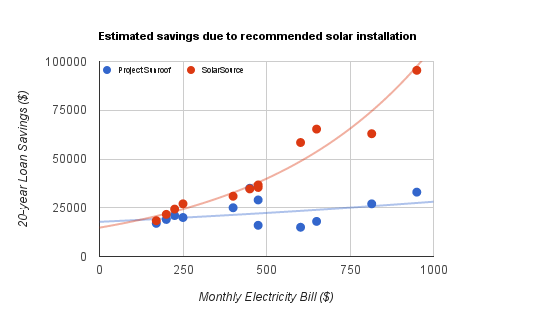
\includegraphics[scale=0.7] {loan-savings}
\caption{Estimated 20-year savings for 12 homes surveyed with Project Sunroof and SolarSource}
\label{fig:loan-savings}
\end{center}
\end{figure}

From the results, we see that our method yields comparable outputs to Project Sunroof for homes with low electricity bills. There is a large discrepancy in estimated savings for homes with high monthly electricity bills. We attribute this discrepancy to the fact that Project Sunroof sets an upper limit of \$500 for monthly bill. Among the twelve homes we tested, four of them had monthly electricity bills that exceeded \$500. For SolarSource, we observe strong exponential correlation between estimated savings and electricity price, with a coefficient of determination value ($R^2$) of .95. What accounts for this strong correlation is likely the fact that while solar array costs increases linearly with installation size, the projected grid electricity costs are compounded exponentially, yielded exponential growth in estimated savings. For Project Sunroof, there is very weak exponential correlation: $R^2 = .16$. We attribute the weak correlation to Project Sunroof's upper limit on electricity bill. Perhaps with a wider range the correlation would be stronger. Figure \ref{fig:loan-savings} demonstrates that our framework yields reasonable cost savings estimates compared to a popular application developed by an established company.

We pass the recommended array capacity and system coordinates as parameters to the PVWatts service. PVWatts requires the caller to provide the module type (standard, premium, or thin film), and system losses. Due to lack of available data, we assume a standard module and 5\% losses, the default value. PVWatts returns an array of monthly AC electricity outputs for the array, which we average for the monthly production. To ascertain generation of the recommended array, we multiply the monthly electricity consumption value (the quotient of electricity bill $b$ and utility rate $u$) by the percentage of consumption $k$ that the array purports to cover. The formula is:

\[ \mbox{array production (kWh/month)} = \frac{b \mbox{ (\$/month) }}{ u \mbox{ (\$/kWh) }} * k (\%) \]

Figure \ref{fig:wattsprod} compares each framework's recommended array production to PVWatts projected production. In this figure each pair of columns represents one surveyed home. The electricity bill for the home is the value used in the analysis. For Project Sunroof, we must use a value of \$500 for homes that exceed the limit.

\begin{figure}[h]
\begin{center}
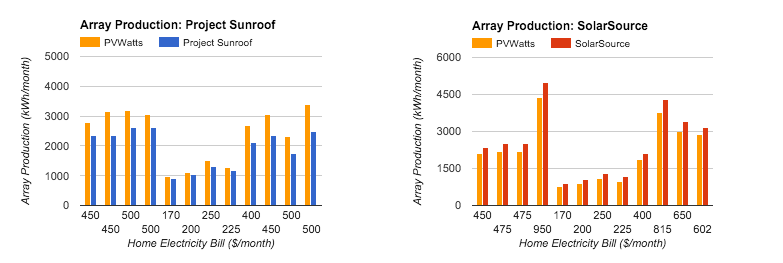
\includegraphics[width = \textwidth] {wattsprod}
\caption{Recommended array production from Project Sunroof and SolarSource compared to PVWatts projection}
\label{fig:wattsprod}
\end{center}
\end{figure}

From the results, we see that Project Sunroof consistently underestimates array production compared to the PVWatts result by an average of -17\%. Oppositely, SolarSource consistently overestimates the value by +15\%. The differing PVWatts generation values for the same homes are due to the different array size recommended by each framework. Though we cannot explain the discrepancy in Project Sunroof underestimation, one potential explanation for SolarSource's overestimation is a high value for power per area from PVDAQ. We expect that using array production data from Enlighten systems (once we obtain access) will improve the accuracy of our implementation in this benchmark.

We use the PVWatts predicted generation values to compute predicted savings. We first multiply the average monthly production value by the electricity rate, then multiply that value by 240 months to yield to gross savings over the 20 year span where we assume that the homeowner saves whatever they don't have to purchase from the utility. From the gross savings value we subtract the array cost. Figure \ref{fig:wattscost} shows the estimated cost savings for each surveyed home reported by Project Sunroof and SolarSource compared to the PVWatts Projected Savings.

\begin{figure}[h]
\begin{center}
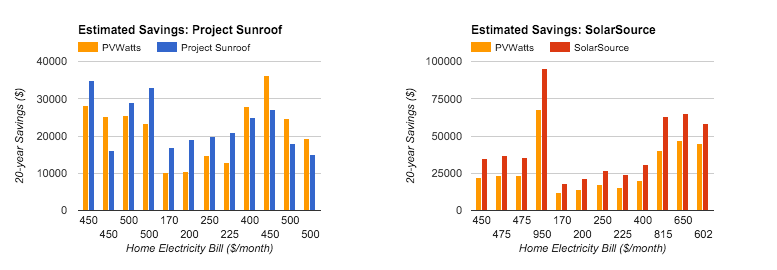
\includegraphics[width = \textwidth] {wattscost}
\caption{Estimated savings fromProject Sunroof and SolarSource compared to PVWatts projection}
\label{fig:wattscost}
\end{center}
\end{figure}

SolarSource consistently overestimates the estimated savings compared to the accepted value by an average of +50\% whereas Project Sunroof sometimes overestimates and sometimes underestimates cost savings, with an average error of 37\%. A high power per area value would again explain SolarSource's overestimation, although it is not definitive. Figure \ref{fig:comparison-table} is a summary of our experiments, reporting the average error between each framework and PVWatts in array production and savings estimate.

\begin{figure}[h]
\begin{center}
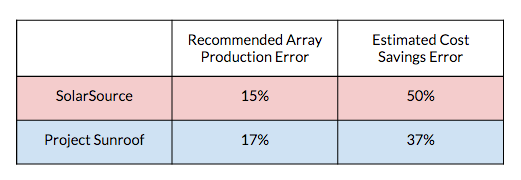
\includegraphics[scale = 0.5] {comp-table}
\caption{Average percent error of SolarSource and Project Sunroof compared to PVWatts in two evaluation metrics}
\label{fig:comparison-table}
\end{center}
\end{figure}

It is worth nothing that SolarSource's accuracy improvement in recommended array production may be a facet of our evaluation methodology. We used the PVWatts projections as the ``true values'' for array production and cost savings. However, PVWatts predictions are not definitively correct; they are projections. Furthermore, as an NREL service, PVWatts may use some of the same underlying data sources as the other NREL services we use in our algorithm. Using the same data sources enhances the likelihood of array output alignment. A more objective comparison could use SolarCast to predict future performance and cost savings. However, as SolarCast is still under development, we settled on PVWatts.

\subsection{Qualitative Comparison}
We have also performed a qualitative analysis of SolarSource compared to Project Sunroof using some of the key principles that guided our approach. Whereas Project Sunroof is only available in 10 US cities, our framework can be used anywhere with internet access as a result of roof and energy profiles created from user-supplied data. 

Project Sunroof lists its assumptions in the estimated savings calculation due to the array; our framework is open source. Anyone user can examine the code on Github to learn how we perform the analyses. We strove to write self-documenting code with a clean structure and descriptive variable names to facilitate understanding.

Although we provide many of the same values at Project Sunroof, we differ in {\em how} we provide that information. Sunroof displays the information in the app's interface. Though visually appealing, the format is inflexible. There is no Project Sunroof API to retrieve the data from the analysis. With a RESTful API backend, we return the information in a JSON object.  A client can make an API request independent of the Android application using an HTTP client like Postman. All that is required is a valid JSON request object as specified on the documentation page. The roof parameters could come from a manual mapping (perhaps with a tape measure, as we used for the Princeton home).  The client can use the returned information however they please. We provide the analysis tools; we don't restrict how the client uses our output.

Project Sunroof cannot be modified or augmented by the open-source community. It uses fixed values for electricity price increase, APR, and future consumption. There is undoubtedly development underway at Google, but there's no way for developers to build on their framework. Google could fathomably open-source the code (the company has a Github organization with over 400 project repository) or release an API as part of its developer program. Currently, however, the code for Sunroof is hidden behind the interface. On the other hand, our code is intended to be ``forked'' on Github. The Node.js framework and our modular architecture enables developers to easily plug in their own modules. Rather than using a fixed value for the assumed electricity price increase, a developer could build her own price forecast model and swap it in to the analysis. Or instead of using the monthly electricity bill as the basis of the analysis, a developer could analyze the Wattvision data stream to determine heaviest hours of use. Without expertise on economic trends or data analytics, we couldn't build advanced models ourselves. But we could create opportunities for people well-versed in those topics to create tools of their own. Our modular architecture and open-source codebase permit that. Figure \ref{fig:qual} is a chart summarizing the qualitative comparison between SolarSource and Project Sunroof.

\begin{figure}[h]
\begin{center}
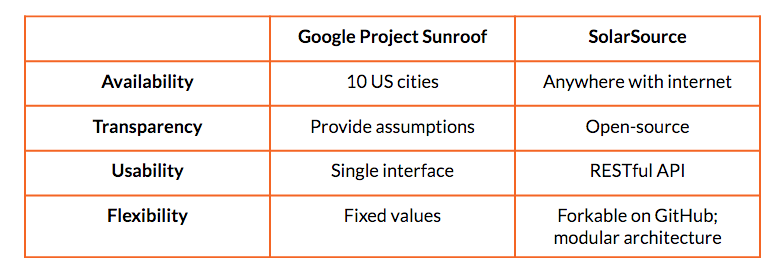
\includegraphics [scale = 0.5] {qual-analysis}
\caption{A qualitative comparison between SolarSource and Project Sunroof in four key categories}
\label{fig:qual}
\end{center}
\end{figure}

\section{Summary}
This paper proposes SolarSource, a universally applicable framework to evaluate rooftop solar potential. A universally applicable framework requires independence from map APIs, flexible access to its analysis tools, and the ability to augment functionality with custom modules. Our calculation of recommended array size is novel in that it uses crowdsourced array production data. The results of our experiments demonstrate that our framework produces reasonable estimates for recommended array size and cost savings. However, using crowdsourced array performance does not greatly improve accuracy of the analysis when compared to existing tools. The primary contribution of our work is the creation of a framework that enables anyone with internet access to compute their home solar potential, provides its analysis tools in the form of a public API, and, through its modular architecture, enables the open-source community to build on the existing foundation. A general and accurate framework helps uncover the financial benefits of solar for the widest audience possible, thereby facilitating the transition to a carbon-free energy future.

We will be presenting the framework and our results to the researchers at the National Renewable Energy Laboratory in February 2016. Sarah Kurtz, the director of the PVDAQ program, is interested in how software developers use NREL's APIs. She sees SolarSource as an ideal use case and asked us to demo the application for her colleagues.

Our system is an early investigation of how to build a solar ``calculator'' as a pluggable, open-source API. As such, it has several limitations, which suggest topics for future work.

The accuracy of our recommendation is limited by our access to atmospheric weather data. For Project Sunroof, Google is able to leverage its proprietary data in historical cloud and temperature patterns that might affect solar energy production. We are limited to public data from sources. In future development, we would look into bolstering the accuracy of our weather information with diversified sources.

Our approach only works for a single, continuous installation. It cannot account for multi-part roofs that face different directions or have different tilt angles. Augmenting the framework to allow for disconnected roofs with different properties is an important step to improve general-purpose use.

Another limitation is that we assume that the panels would be purchased via loan. In actuality, the homeowner could also lease the panels or buy them up front. Building support for various financing options is another key component of our future work.

Enphase Enlighten and PVDAQ both require developer accounts with unique API keys, which we store privately. A developer who forks the SolarSource project on Github does not have API access to either service. In order to enable further development on the project by outside contributors, we must find a workaround to this issue. One potential solution is to store the PVDAQ data statically in a file that we update periodically (once per month, for instance). We don't envision the Enphase data will ever be accessible publicly. Unlike PVDAQ, we can't store the data within the app; in the access authorization email we must state that the user's system generation data will never be published.

Once the SolarCast API is completed we intend to use it both for evaluation and as part of the recommendation algorithm. Rather than assuming the panels will generate electricity at the same capacity for their lifetime, we could incorporate SolarCast's future prediction algorithms to get a more finely-tuned view of lifetime generation potential. That measure would also improve the accuracy of the cost-savings estimate.

Wattvision expressed interest in integrating SolarSource with its existing software suite. Although we intend for the framework to remain general and open source, we could build out a customized version for Wattvision. With that in place, the SolarSource recommendation would be displayed for any Wattvision customer who opts in to discover the cost savings potential of a solar installation.

\bigskip
\bigskip
\bigskip



\begin{center}
\textbf{Acknowledgments}
\end{center}
We are extremely grateful to Alan Kaplan for his guidance and constant support throughout the project's development. We'd also like to thank the Princeton University School of Engineering and Applied Science for its generous funding and the Blejwas family for allowing us to survey their home for testing purposes. We are particularly appreciative of the efforts of Sarah Kurtz at NREL for granting us access to the PVDAQ service and Ben Smith at Enphase for compiling a list of candidate systems and requesting API access on our behalf from Enlighten customers. Lastly we extend our thanks to the Long Island homeowners who provided their electricity billing data.

\bstctlcite{bstctl:etal, bstctl:nodash, bstctl:simpurl}
\bibliographystyle{IEEEtranS}
\bibliography{references}

\end{document}

